\documentclass[class=report, crop=false, 12pt,a4paper]{standalone}
\usepackage{enumitem}
\usepackage{multicol}
\usepackage{graphicx}
\usepackage{float}
\usepackage{amsmath}
\usepackage{amssymb}
\usepackage{mathtools}
\usepackage{siunitx}
\usepackage{commath}
\usepackage{array}
\usepackage{natbib}
\usepackage[a4paper,width=150mm,top=25mm,bottom=25mm]{geometry}
\setlength{\parindent}{0pt}
\begin{document}
\subsection{Statically Determinate Beams}
\begin{center}
  23/10/2020
\end{center}
\textbf{Statically determinate} (or isostatic) beams are characterised by the fact that all unknown supports reactions can be determined from the forces and equilibrium equations: the number of supports reactions is equal to the degree of freedom. \\\\
A beam in 2D plane has 3 DOF. If only lateral loads and moments act (horizontal actions and reactions = 0), the beam has only 2 degree of freedom. \\\\
Beams subjected to lateral loads are statically determinate if they have \textbf{only 2 unknown support reactions:} the two equilibrium equation for lateral forces and moments are sufficient to solve the system. If the supports produce \textbf{three or more unknown reactions}, the beams are \textbf{statically indeterminate}.
\subsection{Double Integration Method}
In more complex cases, such as discontinuous loads, the multiple integration method can still be used:
\begin{enumerate}
  \item Write one bending moment expression for each part of the beam (e.g. $AB$ and $BC$).
  \item Use double integration on each bending moment expression. This would result in 2 constants of integration for each part of the beam (in this case, 4 constants).
  \item Use boundary conditions to determine constant of integration.
\end{enumerate}
The boundary conditions at the supports are generally not sufficient to obtain all the constants of integration (in our case we need 4 and they are 2) $\therefore$ We need other boundary conditions.
\subsubsection{Example: Concentrated Load on a Simply Supported Beam}
\begin{figure}[H]
  \centering
  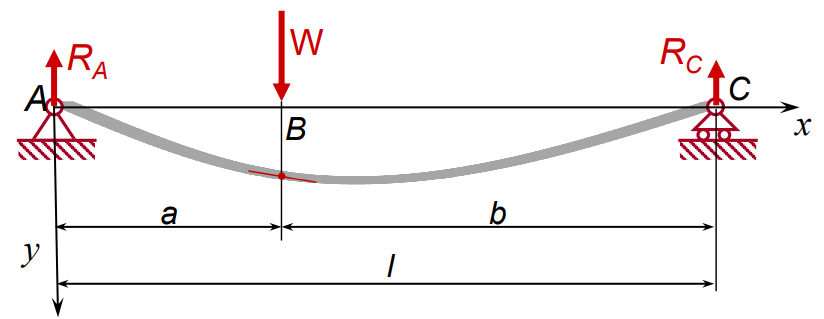
\includegraphics[width = 0.75 \textwidth]{../img/beam6.PNG}
\end{figure}
We know that, tough the load is discontinuous; the slope and deflection of the beam must be continuous from one section to the next. $\therefore$ at C:
\begin{gather}
  \theta_{AC} = \theta_{CB} \\
  y_{AC} = y_{CB}
\end{gather}
The 1st equation refers to continuous slope, while the 2nd equation refers to continuous deflection. Continuity of slope and deflection of the beam from adjacent sections provides the supplementary equations that allow us to determine all constant of integration. By solving the system of equations, the following can be obtained: 
\begin{gather}
  y_a = -\frac{x}{6EIl}[R_Al(x^2-l^2)+W(l-a)^3] \\
  y_b = -\frac{1}{6EIl}[R_Alx(x^2-l^2)-Wl(x-a)^3+Wx(l-a)^3]
\end{gather}
Memorising or fully understanding these equations are not that important; it is more crucial to understand the whole process of double integration method. \\\\
If a system is composed of $n$ parts:
\begin{itemize}[noitemsep]
  \item Determine $n$ equations of the bending moment
  \item Solve $2n$ integrals
  \item Solve a system of $2n$ equations in $2n$ unknowns
\end{itemize}
\section{Macaulay’s Method}
\subsection{Step Function}
We define the step function:
\[ 
  \langle x-a \rangle^n =   
  \begin{cases} 
    (x-a)^n & x-a\geq 0 \\
    0 & x-a<0 
  \end{cases}
\]
The step function can easily describe the common forms of bending moment distribution. The expression of the bending moment can be obtained, moving from the left extreme of the beam to the right, adding every time we find a new load the quantities:
\begin{figure}[H]
  \centering
  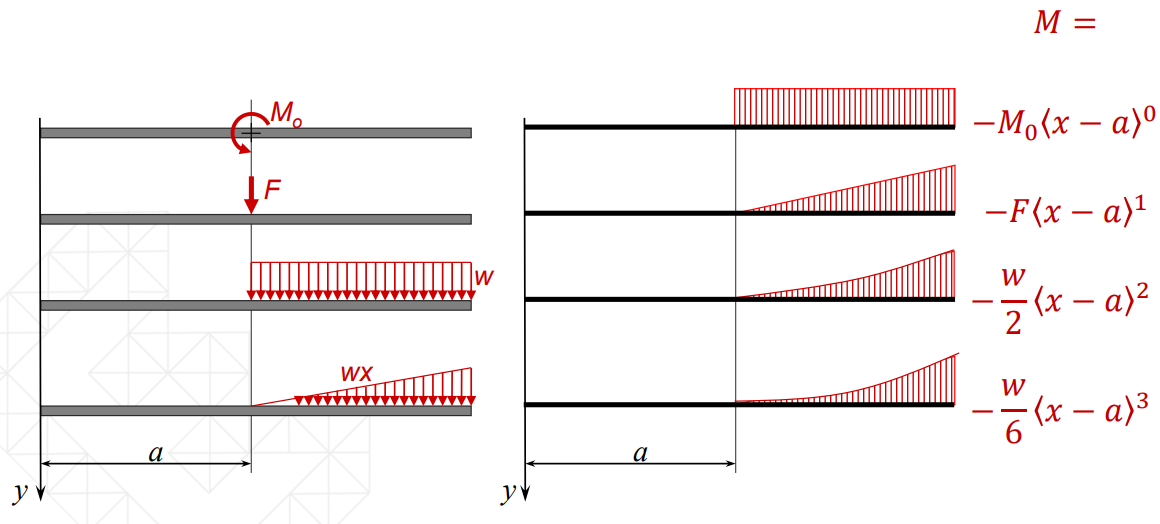
\includegraphics[width = 1 \textwidth]{../img/beam7.PNG}
  \caption{Different loads/moments applied to beams, their respective moment distributions and step functions}
\end{figure}
The crucial property of the step function is that it can be integrated just like an ordinary polynomial expression: 
\begin{gather}
  \int \langle x-a \rangle^n \dif x = \frac{\langle x-a \rangle^{n+1}}{n+1} + C
\end{gather}
Using the step function, the expressions of the different parts of a beam (under discontinuous load) can be put together into one single expression.
\subsubsection{Example: Simply Supported Beam with a Concentrated Load}
\begin{figure}[H]
  \centering
  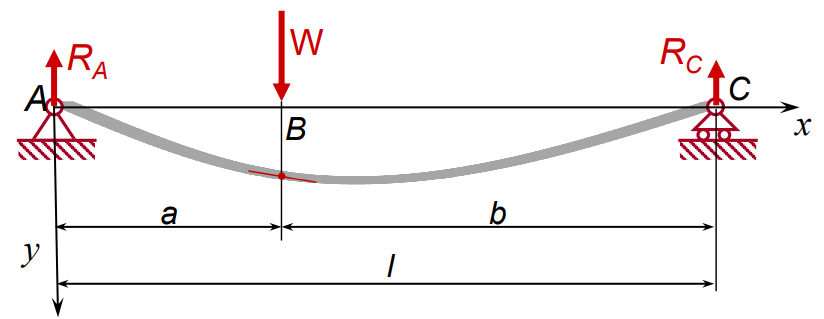
\includegraphics[width = 0.75 \textwidth]{../img/beam6.PNG}
\end{figure}
The bending distribution in AB and BC respectivelty is:
\begin{gather}
  M_a = R_Ax \\
  M_b = R_Ax - W(x-a)
\end{gather}
Using the step function, the bending distribution in the entire beam is:
\begin{gather}
  M = R_Ax - W\langle x-a \rangle \\
  \theta = -\frac{1}{EI}\int M \dif x = -\frac{1}{EI}\left[R_A+\int x \dif x - W\int \langle x-a \rangle \dif x \right] \\
  = -\frac{1}{EI}\left(\frac{R_Ax^2}{2}-\frac{W\langle x-a \rangle^2}{2}\right) + \theta_0 \\
  y = \int \theta \dif x = -\frac{1}{EI}\left[\frac{R_Ax^3}{6}-\frac{W\langle x-a \rangle^3}{6}\right] + \theta_0x + y_0
\end{gather}
There are only 2 integration constants $\therefore$ 2 boundary conditions are sufficient to solve the equation.
\subsection{Examples}
The following figures and equations are just examples of generic loads on simply supported beams, and what their step functions are. To find the deflection, the functions need to be integrated twice, and the boundary conditions must be substituted to find the integration constants.
\begin{figure}[H]
  \centering
  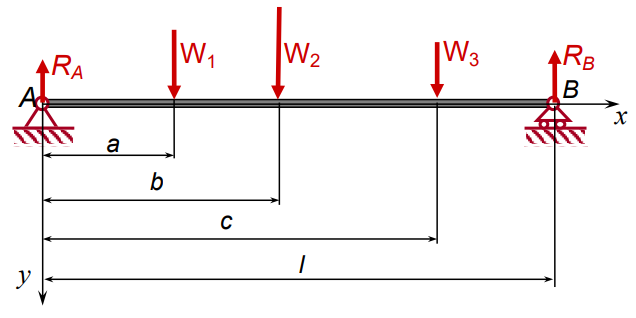
\includegraphics[width = 0.65 \textwidth]{../img/beam8.PNG}
\end{figure}
\begin{gather}
  M = R_Ax - W_1\langle x-a \rangle - W_2\langle x-b \rangle - W_3\langle x-c \rangle 
\end{gather}
\begin{figure}[H]
  \centering
  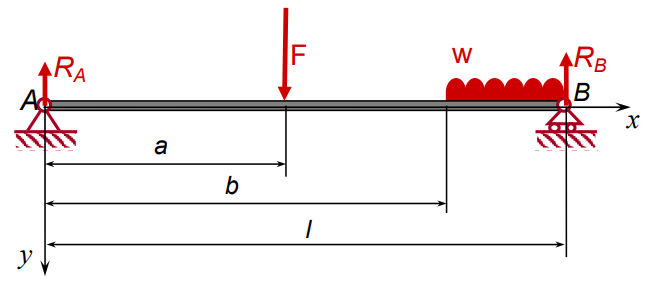
\includegraphics[width = 0.7 \textwidth]{../img/beam9.PNG}
\end{figure}
\begin{gather}
  M = R_Ax - F\langle x-a \rangle - \frac{w}{2}\langle x-b \rangle^2
\end{gather}
\begin{figure}[H]
  \centering
  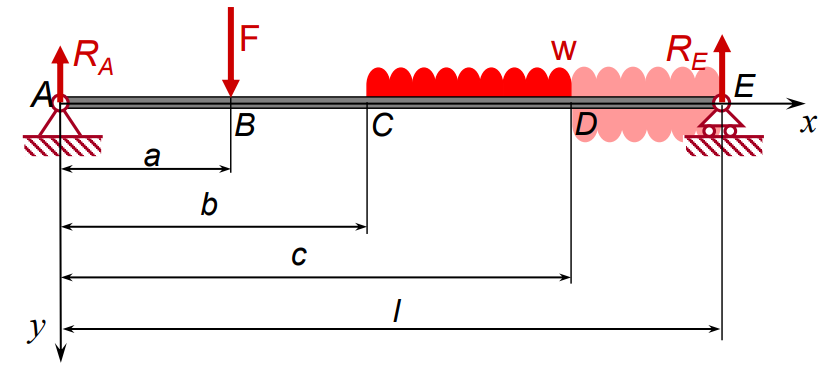
\includegraphics[width = 0.65 \textwidth]{../img/beam10.PNG}
\end{figure}
In this example, the distributed load is not acting all the way to the end point E $\therefore$ A counteracting distributed load is added to cancel the contribution of the distributed load between DE.
\begin{gather}
  M = R_Ax - F\langle x-a \rangle - \frac{w}{2}\langle x-b \rangle^2 + \frac{w}{2}\langle x-c \rangle^2
\end{gather}
\end{document}